\chapter{CVA Calculation for an Interest Rate Swap}\label{chap:cva}

The credit value adjustment (CVA) measures the counterparty credit risk (CCR) in aims of regulation and accounting and pricing purposes. The needs for CVA lie on

\begin{itemize}
  \item Existence of variation on couterparty's credit rating;
  \item The variation causes uncertainty to future expected value of the instrument's accounting CVA;
  \item The uncertainty causes potential MtM losses.
\end{itemize}

In this project, I calculate the CVA of a swap portfolio of an imaginary investment bank and particularly the CVA of a swap given in context.  

The formula of CVA is 
$$
CVA(t,T) = LGD \int_t^T EE(u) d PD_C(c)
$$
where $LGD=(1-RR)$ is the loss given default, $EE$ is the discounted expected exposure, and $PD$ is the default probability. 

\section{Swap Portfolio}
Consider a trading book of an investment book that contains 31 swaps with 6 counterparties. The swap book specifications are shown in Table~\ref{table::swap_port}. The swap position with our particular interest is the last one, with 1 million dollar notional value and 5-Yr maturity. The unique couterparty of this swap is 6, different with all other swaps.

\begin{center}
\scalebox{0.7}{
\begin{tabular}{|c|c|c|c|c|c|c|c|c|} 
  \hline
  CounterpartyID	&	NettingID	&	Principal	&	Maturity	&	LegType	&	LegRateReceiving	&	LegRatePaying	&	LatestFloatingRate	&	Period	\\ \hline
5	&	5	&	813450	&	13-Dec-17	&	1	&	0.036134726	&	10	&	0.03462651	&	1	\\
5	&		&	441321	&	26-Oct-17	&	0	&	87	&	0.039251637	&	0.033598155	&	1	\\
1	&		&	629468	&	4-Sep-20	&	1	&	0.038682219	&	0	&	0.035674961	&	1	\\
5	&		&	774308	&	2-Mar-22	&	0	&	70	&	0.046303151	&	0.035364042	&	1	\\
4	&		&	918177	&	4-Feb-23	&	1	&	0.047524758	&	74	&	0.034985981	&	1	\\
1	&	1	&	969469	&	10-Apr-18	&	0	&	78	&	0.040000628	&	0.03497566	&	1	\\
2	&	2	&	660412	&	27-Nov-20	&	0	&	8	&	0.0395239	&	0.034441285	&	1	\\
3	&		&	353968	&	23-Apr-20	&	1	&	0.041441865	&	36	&	0.03571308	&	1	\\
5	&	5	&	361971	&	26-Jul-17	&	1	&	0.036346283	&	23	&	0.034906748	&	1	\\
5	&		&	443131	&	8-Jul-19	&	0	&	72	&	0.042262413	&	0.034499829	&	1	\\
1	&		&	880538	&	20-Jun-18	&	1	&	0.038769776	&	39	&	0.03594597	&	1	\\
5	&		&	440712	&	4-Apr-22	&	1	&	0.047340175	&	82	&	0.03484266	&	1	\\
5	&	5	&	860714	&	13-May-19	&	0	&	16	&	0.038394576	&	0.03458768	&	1	\\
3	&	3	&	432644	&	30-Aug-20	&	0	&	24	&	0.040345451	&	0.034794372	&	1	\\
5	&		&	946948	&	28-Jun-18	&	0	&	13	&	0.03672928	&	0.034406452	&	1	\\
1	&		&	512488	&	7-Feb-21	&	0	&	12	&	0.040163882	&	0.03421591	&	1	\\
3	&		&	397446	&	27-Jan-19	&	1	&	0.042759613	&	78	&	0.0367682	&	1	\\
5	&	5	&	438313	&	1-Jun-21	&	1	&	0.044307315	&	52	&	0.036158848	&	1	\\
4	&	4	&	712034	&	17-Aug-21	&	1	&	0.043550797	&	49	&	0.035215275	&	1	\\
5	&	5	&	604967	&	24-Dec-21	&	1	&	0.041084165	&	13	&	0.034120017	&	1	\\
4	&		&	513745	&	13-Mar-20	&	1	&	0.043913829	&	77	&	0.034394172	&	1	\\
1	&	1	&	873121	&	31-Dec-17	&	0	&	56	&	0.038559439	&	0.034876426	&	1	\\
5	&	5	&	688948	&	13-Nov-18	&	1	&	0.039015461	&	32	&	0.035553991	&	1	\\
5	&		&	662293	&	21-Dec-22	&	1	&	0.044799911	&	46	&	0.034067597	&	1	\\
4	&		&	937895	&	30-May-18	&	0	&	36	&	0.037257157	&	0.033369093	&	1	\\
4	&		&	464379	&	13-Jun-22	&	1	&	0.041390133	&	7	&	0.033985632	&	1	\\
4	&	4	&	817900	&	21-Sep-20	&	1	&	0.040423141	&	22	&	0.035233458	&	1	\\
2	&		&	815297	&	21-Jun-23	&	1	&	0.04294236	&	11	&	0.035273948	&	1	\\
4	&	4	&	535334	&	18-Dec-17	&	1	&	0.036839018	&	17	&	0.035316176	&	1	\\
1	&		&	675866	&	24-Feb-20	&	1	&	0.039916611	&	22	&	0.034908801	&	1	\\
6	&	6	&	1.00E+06	&	30-Jun-21	&	1	&	0.036134726	&	10	&	0.03462651	&	1	\\
  \hline
\end{tabular}}\label{table::swap_port}
\end{center}

The credit spread dynamics over the next 5 years are shown in Table~\ref{table::swap_port}. The unit of these credit spreads is per basis point. For the 5-Yr swap of our interest, I assume a flat credit spread with 200 basis points over the risk-free rate.

\begin{center}
\begin{tabular}{|c|c|c|c|c|c|c|} 
  \hline
Date	&	cp1	&	cp2	&	cp3	&	cp4	&	cp5	&	cp6	\\ \hline
6/30/2017	&	140	&	85	&	115	&	170	&	140	&	200	\\
6/30/2018	&	185	&	120	&	150	&	205	&	175	&	200	\\
6/30/2019	&	215	&	170	&	195	&	245	&	210	&	200	\\
6/30/2020	&	275	&	215	&	240	&	285	&	265	&	200	\\
6/30/2021	&	340	&	255	&	290	&	320	&	310	&	200	\\
  \hline
\end{tabular}\label{table::credit_spread}
\end{center}

\section{Market Environment}
I chose the market date 2016-06-30 and download the swap rates from Bloomberg. The zero rates from the market is shown in Figure~\ref{fig::cva_zero_rate}. 

\begin{center}
  \begin{figure}
  \centering
      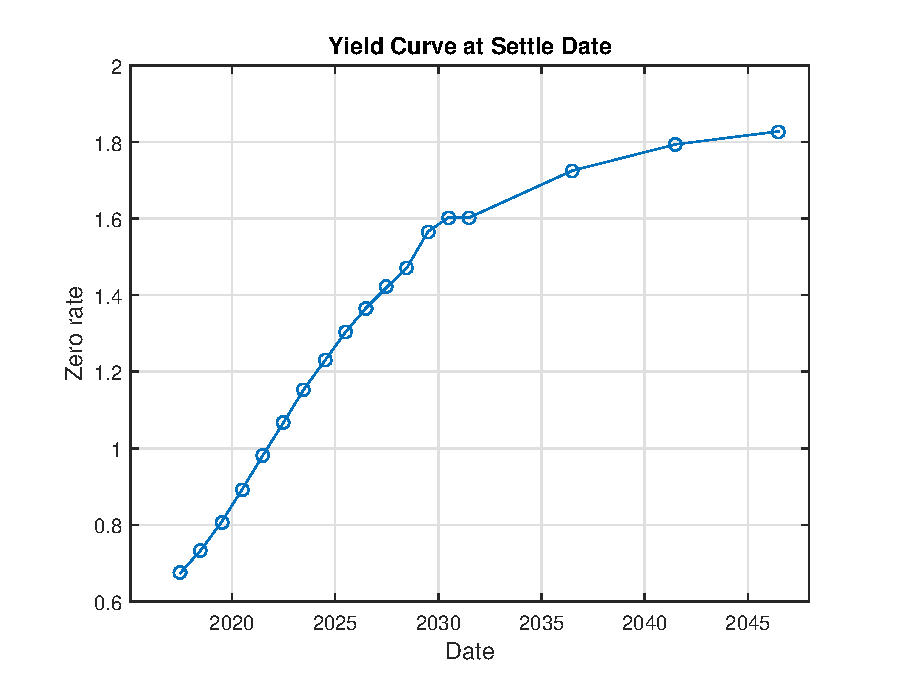
\includegraphics[scale=0.6]{cva_zero_rate.eps}
      \caption{The zero rate as of 2016-06-30 from Bloomberg.}\label{fig::cva_zero_rate}
  \end{figure}
\end{center} 

To populate market consistent interest rate scenarios, a Hull-White one factor model is fitted with $a=0.2$ and $\sigma=0.015$. Therefore, the model specification is 
$$
dr = [\theta(t)-ar] dt +\sigma dW(t)
$$
where
$$
\theta(t) = f_t(0,t) + a f_t(0,t) + \frac{\sigma^2}{a}(1-e^{-2at}) 
$$

For a randomly selected scenario, the yield curve evolution is shown in Figure~\ref{fig::cva_yield_curve}. 

\begin{center}
  \begin{figure}
  \centering
      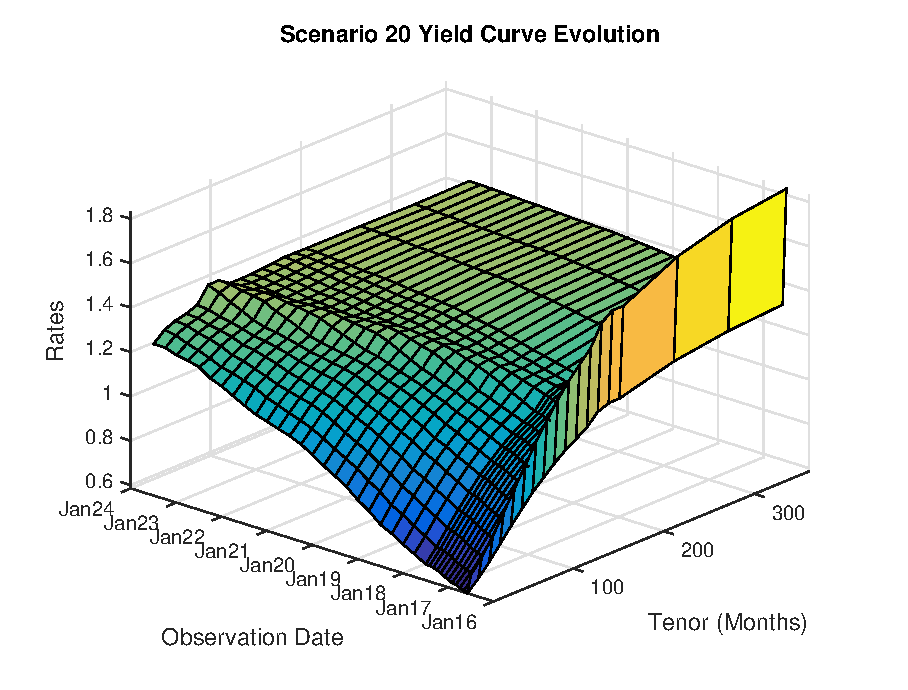
\includegraphics[scale=0.6]{cva_yield_curve.eps}
      \caption{Yield curve evolution at scenario 20.}\label{fig::cva_yield_curve}
  \end{figure}
\end{center} 

\section{CVA Calculation}
Using the Hull-White model projected scenarios to price the swap, the mark-to-market portfolio value on the 5-Yr swap can be calculated. Note that for easier comparison and illustration, I make the notional of the swap to 1,000,000. Figure~\ref{fig::cva_mtm_value}.

\begin{center}
  \begin{figure}
  \centering
      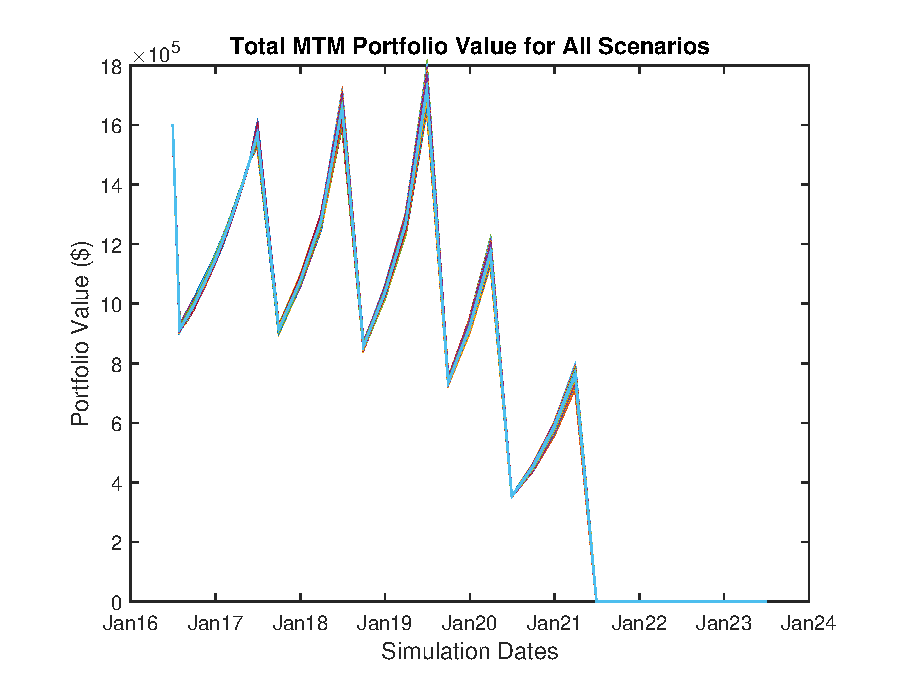
\includegraphics[scale=0.6]{cva_mtm_value.eps}
      \caption{Mark-to-market value of the swap over projection periods.}\label{fig::cva_mtm_value}
  \end{figure}
\end{center} 

The exposure profile of the swap is plotted in Figure~\ref{fig::cva_exposure_profile}. The exposure over time, location of maximum exposure and potential future exposure at 95\%  are calculated and shown in the graph. 

\begin{center}
  \begin{figure}
  \centering
      \includegraphics[scale=0.6]{cva_exposure_profile.eps}
      \caption{Mark-to-market value of the swap over projection periods.}\label{fig::cva_exposure_profile}
  \end{figure}
\end{center} 

The probability of default for each counterparty is bootstrapped from the credit spreads, and its dynamic over time is plotted in Figure~\ref{fig::cva_default_prob}.

\begin{center}
  \begin{figure}
  \centering
      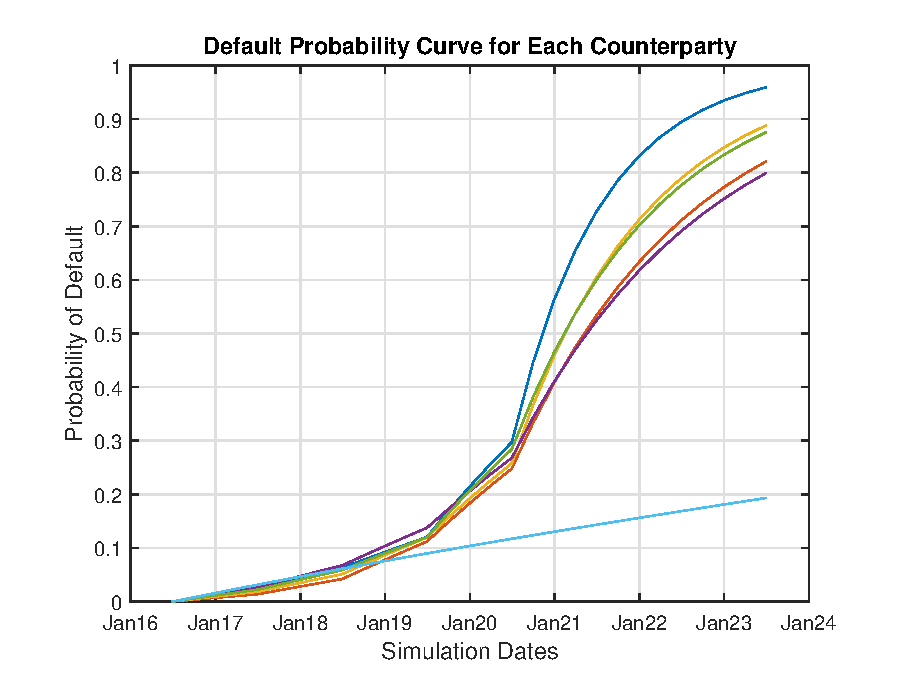
\includegraphics[scale=0.6]{cva_default_prob.eps}
      \caption{Probability probabilities bootstrapped from the credit spreads.}\label{fig::cva_default_prob}
  \end{figure}
\end{center}

Finally, the CVA is calculated by a finite sum over the valuation dates.
$$
CVA = (1-RR)\sum_{i=2}^n EE(T_i) [PD(T_i)-PD(T_{i-1})]
$$

The CVA of the swap with 1,000,000 notional and credit spread assumption is 29054.76. The CVA for each counterparty is shown in Figure~\ref{fig::cva_calc}.

\begin{center}
  \begin{figure}
  \centering
      \includegraphics[scale=0.6]{cva_calc.eps}
      \caption{The CVA calculation for each counterparty in the swap book.}\label{fig::cva_calc}
  \end{figure}
\end{center}